\chapter{Resultat}\label{cha:Research}
%
Det här är kapitlet där resultaten presenteras.


\section{Ditten}\label{sec:research:history}
%
Liksom \citep{Duck:2005} har vi kommit fram till att glass smakar bäst på sommaren.

\marginpar{Kommer att tänka på en liten anekdot\ldots}

\Warning[TODO]{Ta bort den löjliga anekdoten!}

När vi nu går in på hur glass smakar vid olika tidpunkter under dagen hänvisar vi till \figureref{fig:times}, och speciellt till \figureref{fig:times:early}.  Jämför sedan med \figureref{fig:times2} för att se hur det kan bli när man äter glass vid okontrollerade tidpunkter.

Veselić, Krešimir (Veseli\'{c}, Kre\v{s}imir) skrev en gång en artikel med titeln \emph{Bounds for exponentially stable semigroups}.

\begin{figure}[tbp]
  \centering
  \subfloat[Alldeles för tidigt.][\label{fig:times:very-early}Det här är väl tidigt — din glass hinner smälta innan ditt sällskap dyker upp.]{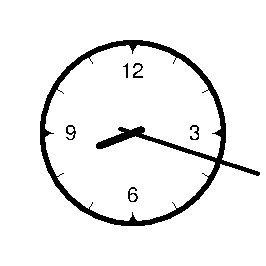
\includegraphics[page=1]{clocks}}
  \qquad
  \subfloat[Med marginal.][\label{fig:times:early}Kiosken stänger snart, men inte nu — perfekt!]{\includegraphics[page=2]{clocks}}
  \\
  \subfloat[I grevens tid.][\label{fig:times:on-time}Precis i tid — du får in ett finger i luckan just när kiosken ska stänga.  Han som jobbar blir sur, och det blir smolk i bägaren.]{\includegraphics[page=3]{clocks}}
  \qquad
  \subfloat[Försent.][\label{fig:times:late}Du är sen — kiosken är stängd.]{\includegraphics[page=4]{clocks}}
  \caption{\label{fig:times}%
    Illustration av \emph{subfloats}.  Den så kallade \emph{bounding box}en visas i \protect\subref{fig:times:late}.  Lägg märke till att bounding boxen har satts så att alla bilder har samma storlek, med enhetlig placering av själva innehållet i förhållande till bounding boxen.  Antag att du ska träffa en kompis för att äta glass just när kiosken stänger för dagen vid 08:30.  När dyker du upp?}
\end{figure}

\begin{figure}[tbp]
  \centering
  \subfloat[][\label{fig:times2:very-early}]{\includegraphics[page=5]{clocks}}
  \qquad
  \subfloat[][\label{fig:times2:early}]{\includegraphics[page=6]{clocks}}
  \\
  \subfloat[][\label{fig:times2:on-time}]{\includegraphics[page=7]{clocks}}
  \qquad
  \subfloat[][\label{fig:times2:late}]{\includegraphics[page=8]{clocks}}
  \caption{\label{fig:times2}%
    En andra illustration av \emph{subfloats}.  Den här gången har bounding boxen gjorts så liten som möjligt runt själva innehållet.  Resultatet är stökiga placeringar på sidan.  Samma sak kan hända med vanliga fyrkantiga figurer när man har text som spretar ut åt lite olika håll från själva rutan med kurvor i.}
\end{figure}

\section{Framtiden}

Sen när glassen är uppäten är det bara till att sätta igång och skriva på exjobbet igen!


\begin{chapter-appendix}

\section{Ett par långa bevis}
%
Det här är en appendix-del av det aktuella kapitlet.

\end{chapter-appendix}
